\documentclass{beamer}

\usetheme{default}
\usecolortheme{default}

\title{File Sharing using Cryptographically Enforced Access Control}
\author{Daniel Randall}
\institute{Imperial College London}
\date{24th June, 2013}



\begin{document}

\maketitle
  
  % problem slide	
  \begin{frame}
    \frametitle{The problem}
    \framesubtitle{How to share files with multiple groups using existing solutions}
    %Content goes here
    Share a file with different groups of friends using Dropbox, Wuala, Mega:
    \begin{columns}[t] % contents are top vertically aligned
     \begin{column}[T]{3cm}
     \begin{center}
     
\includegraphics[scale=0.2]{images/file/jpgicon.png} \\
     $\boldsymbol{\downarrow}$ \\
     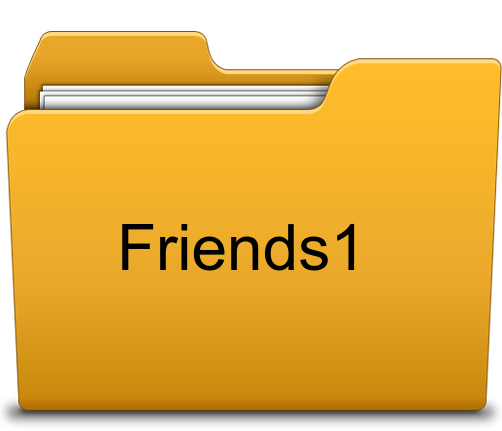
\includegraphics[scale=0.15]{images/folder/friends1}
     \end{center}
     \end{column}
     
     \begin{column}[T]{3cm}
     \begin{center}
     
\includegraphics[scale=0.2]{images/file/jpgicon.png} \\
     $\boldsymbol{\downarrow}$ \\
     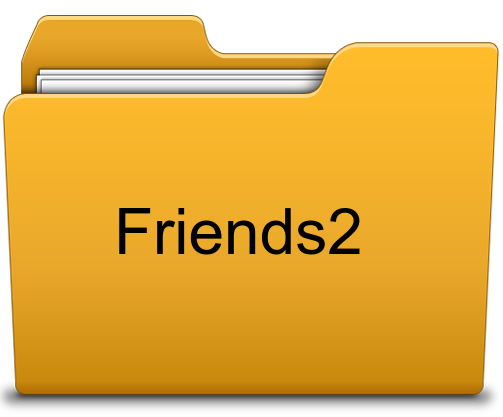
\includegraphics[scale=0.15]{images/folder/friends2}
     \end{center}
     \end{column}
     
     \begin{column}[T]{3cm}
     \begin{center}
     
\includegraphics[scale=0.2]{images/file/jpgicon.png} \\
     $\boldsymbol{\downarrow}$ \\
     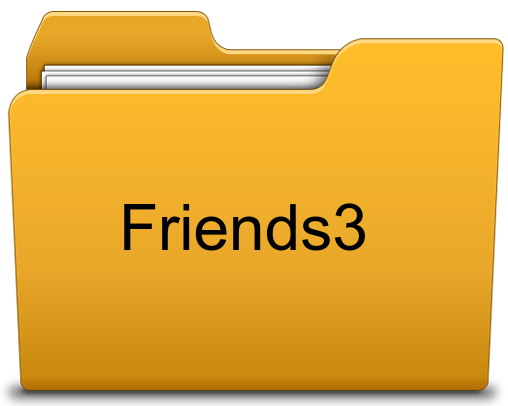
\includegraphics[scale=0.15]{images/folder/friends3}       
     \end{center} 
     \end{column}

     \end{columns}
  \end{frame}
  
  % proposed solution slide
  \begin{frame}
    \frametitle{Proposed solution}
    %Content goes here
    Each file and friend are assigned a rank and the files are automatically transferred to the correct groups \\
    \vspace*{0.5cm}
   \begin{center}
    Files flow upwards $\boldsymbol{\longrightarrow}$
    \vspace*{-1cm}
   \end{center}
    \begin{columns}
    \begin{column}[T]{1cm}
     \begin{center}
      \textbf{Low} 
     \end{center} 
     \end{column}
     
     \begin{column}[T]{1cm}
     \begin{center}
      5
     \end{center} 
     \end{column}

     \begin{column}[T]{1cm}
     \begin{center}
     4
     \end{center} 
     \end{column}
     
     \begin{column}[T]{1cm}
     \begin{center}
      3
     \end{center} 
     \end{column}
     
     \begin{column}[T]{1cm}
     \begin{center}
      2
     \end{center} 
     \end{column}
     
     \begin{column}[T]{1cm}
     \begin{center}
      1
     \end{center} 
     \end{column}
     
     \begin{column}[T]{1cm}
     \begin{center}
      \textbf{High}
     \end{center} 
     \end{column}
    \end{columns}
    \vspace*{1.5cm}
    Therefore, Group5 $\subseteq$ Group4 $\subseteq$ Group3 ...
  \end{frame}
%  \begin{itemize}
%  	\item Users generate a key for each level they can assign files to \\
%  	\item When a file is shared, the file is encrypted the corresponding key \\
%  	\item Friend can derive each key for the level they have access to and use %that to decrypt the file
%  	\end{itemize}
  \begin{frame}
  	\frametitle{How we achieve this}
  	\framesubtitle{Cryptography}
  	File labelled with a label $x$ and the file is encrypted and shared with friends with label y, $y \leq x$. Example:
  	\begin{center}
 		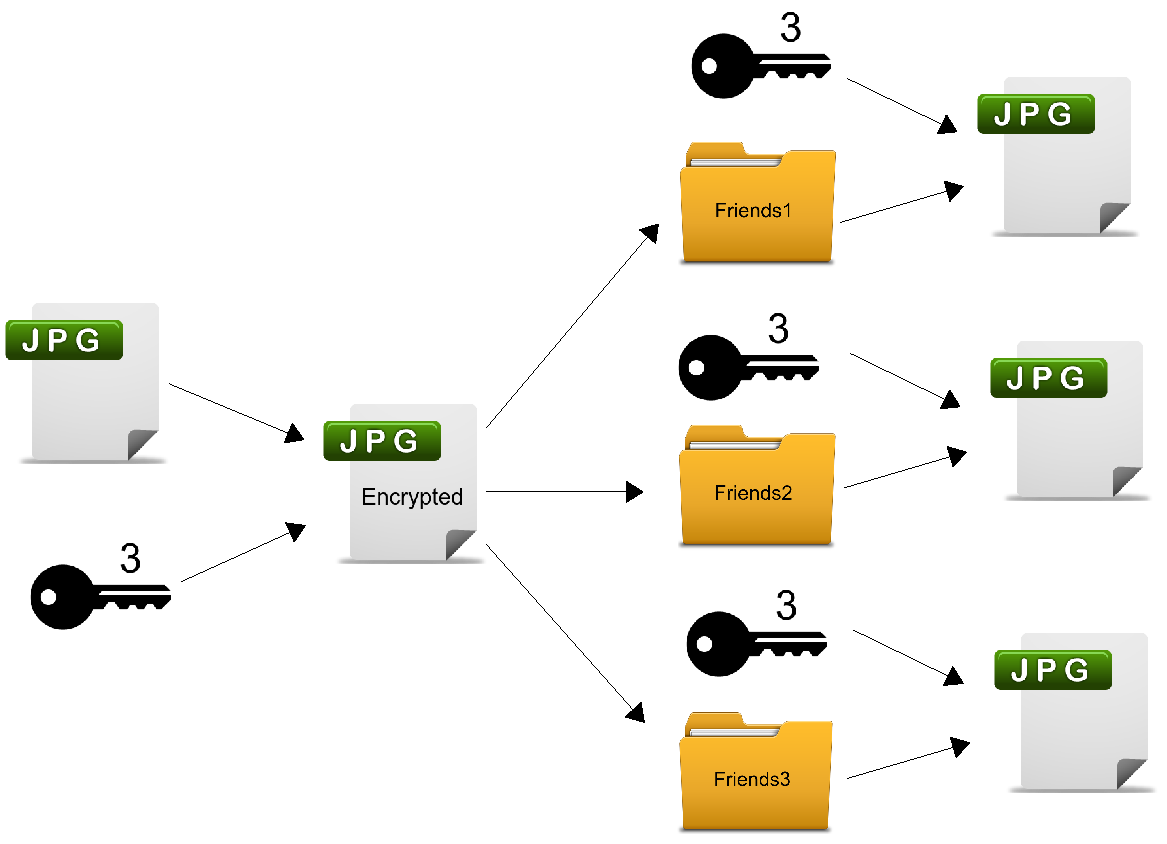
\includegraphics[scale=0.40]{images/sharing/sharing_scissored.pdf}
 	\end{center}
  	
  \end{frame}
  
  \begin{frame}
  	\frametitle{How we store keys}
  	\framesubtitle{Hierarchical cryptography}
  	\begin{center}
  		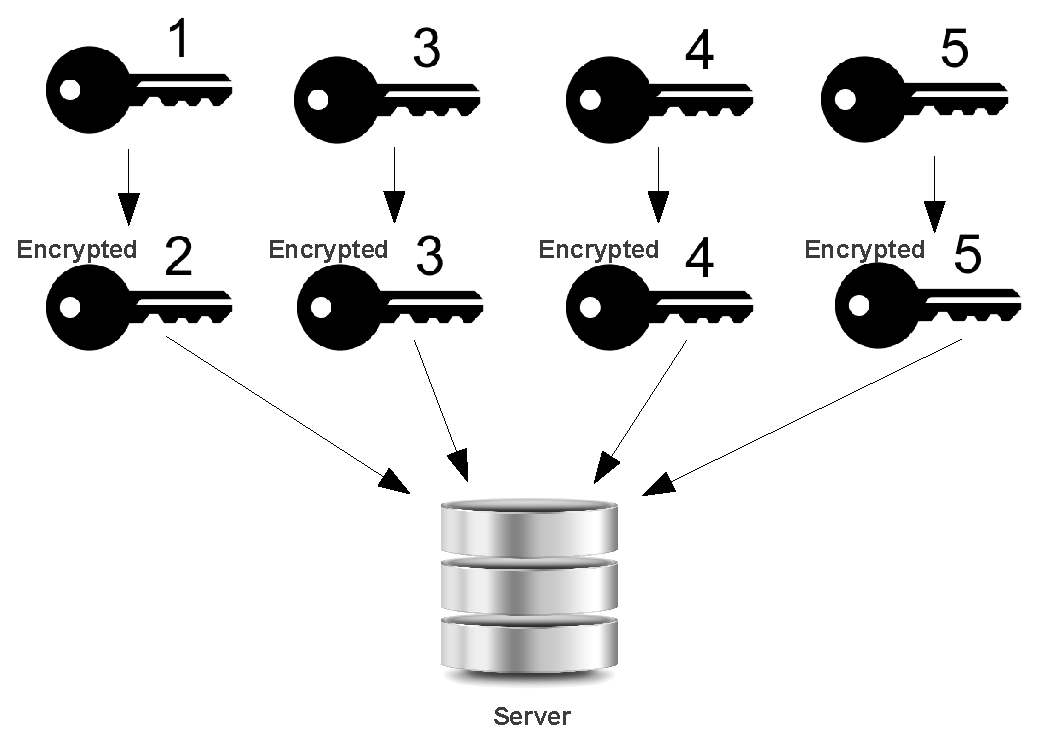
\includegraphics[scale=0.5]{images/keyStorage/keyStorage_scissored.pdf}
  	\end{center}
  \end{frame}
  
  
  % key derivation
  \begin{frame}
  \frametitle{How we derive keys}
  \framesubtitle{Hierarchical cryptography}
  \begin{center}
  	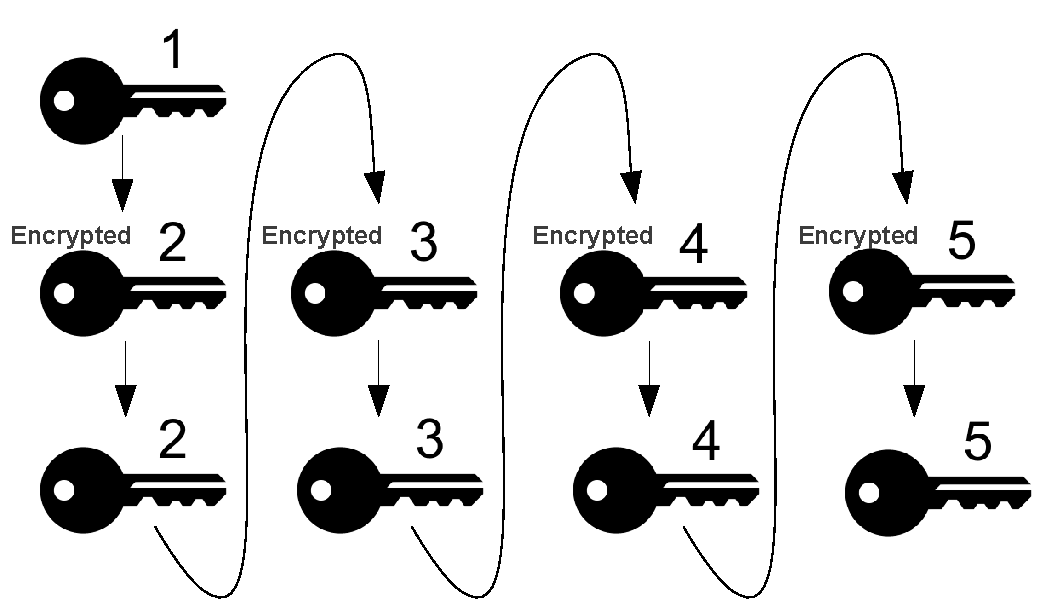
\includegraphics[scale=0.55]{images/keyDerivation/keyDerivation_scissored.pdf}
  \end{center}
  \end{frame}
  
  \begin{frame}
  	\frametitle{How keys are shared}
  	\framesubtitle{Public key cryptography}
  	\begin{center}
  		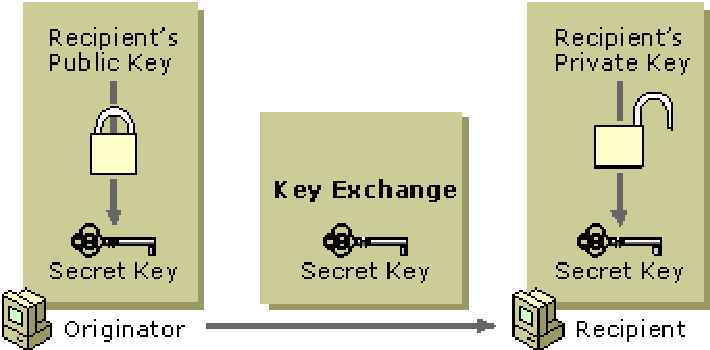
\includegraphics[scale=0.65]{images/publicKey/rsaKeyExchange.pdf}
  	\end{center}
  \end{frame}
  
  \begin{frame}
  	\frametitle{Updating files}
  	
  \end{frame}
  
  
  \begin{frame}
	\frametitle{Revoking users}
	When a user no longer wishes to share files with a friend with access level $x$...
	\begin{itemize}
		\item Replace keys with level y, where $y \leq x$
		\item Re-encrypt files with level y, where $y \leq x$
		\item Re-share new keys with friends that still have access
	\end{itemize}
  \end{frame} 
  
  
  %usefulness
  \begin{frame}
  	\frametitle{Applications}
  	Useful in work environments:
  	\begin{columns}
  		\begin{column}[T]{4cm}
	 	 	\begin{itemize}
	 	 		\itemsep1em
  				\item Project manager
  				\item Project member
  				\item Project intern
 			\end{itemize}
		\end{column}
	
		\begin{column}[T]{1cm}
			\vspace*{1cm}
			$\boldsymbol{\longrightarrow}$
			
		\end{column}
	
		\begin{column}[T]{4cm}
			\begin{block}{Level 1}
				Project manger
			\end{block}
			\begin{block}{Level 2}
				Project member
			\end{block}
			\begin{block}{Level 3}
				Project intern
			\end{block}
		\end{column}
 	
  	\end{columns}
  	\vspace*{0.3cm}
 	 Not so clearly useful in social environments: 
  	\begin{columns}
  		\begin{column}[T]{4cm}
	 	 	\begin{itemize}
  				\item Mum
  				\item Friend
  				\item Uncle
 			\end{itemize}
		\end{column}
	
		\begin{column}[T]{1cm}
			\vspace*{1cm}
			$\boldsymbol{\longrightarrow}$
		\end{column}
	
		\begin{column}[T]{4cm}
			\vspace*{1cm}
			?
		\end{column}
		\end{columns}
  
  \end{frame}
  
  
  
  \begin{frame}
  	\frametitle{Future work}
  	\framesubtitle{Multiple hierarchies}
  	
  \end{frame}
  
  \begin{frame}
  	\frametitle{Future work}
  	\framesubtitle{Adjustable lower bounds}
  	Lowest assigned bound does not have to be the lowest available (i.e. 5)
  	\begin{center}
 	 	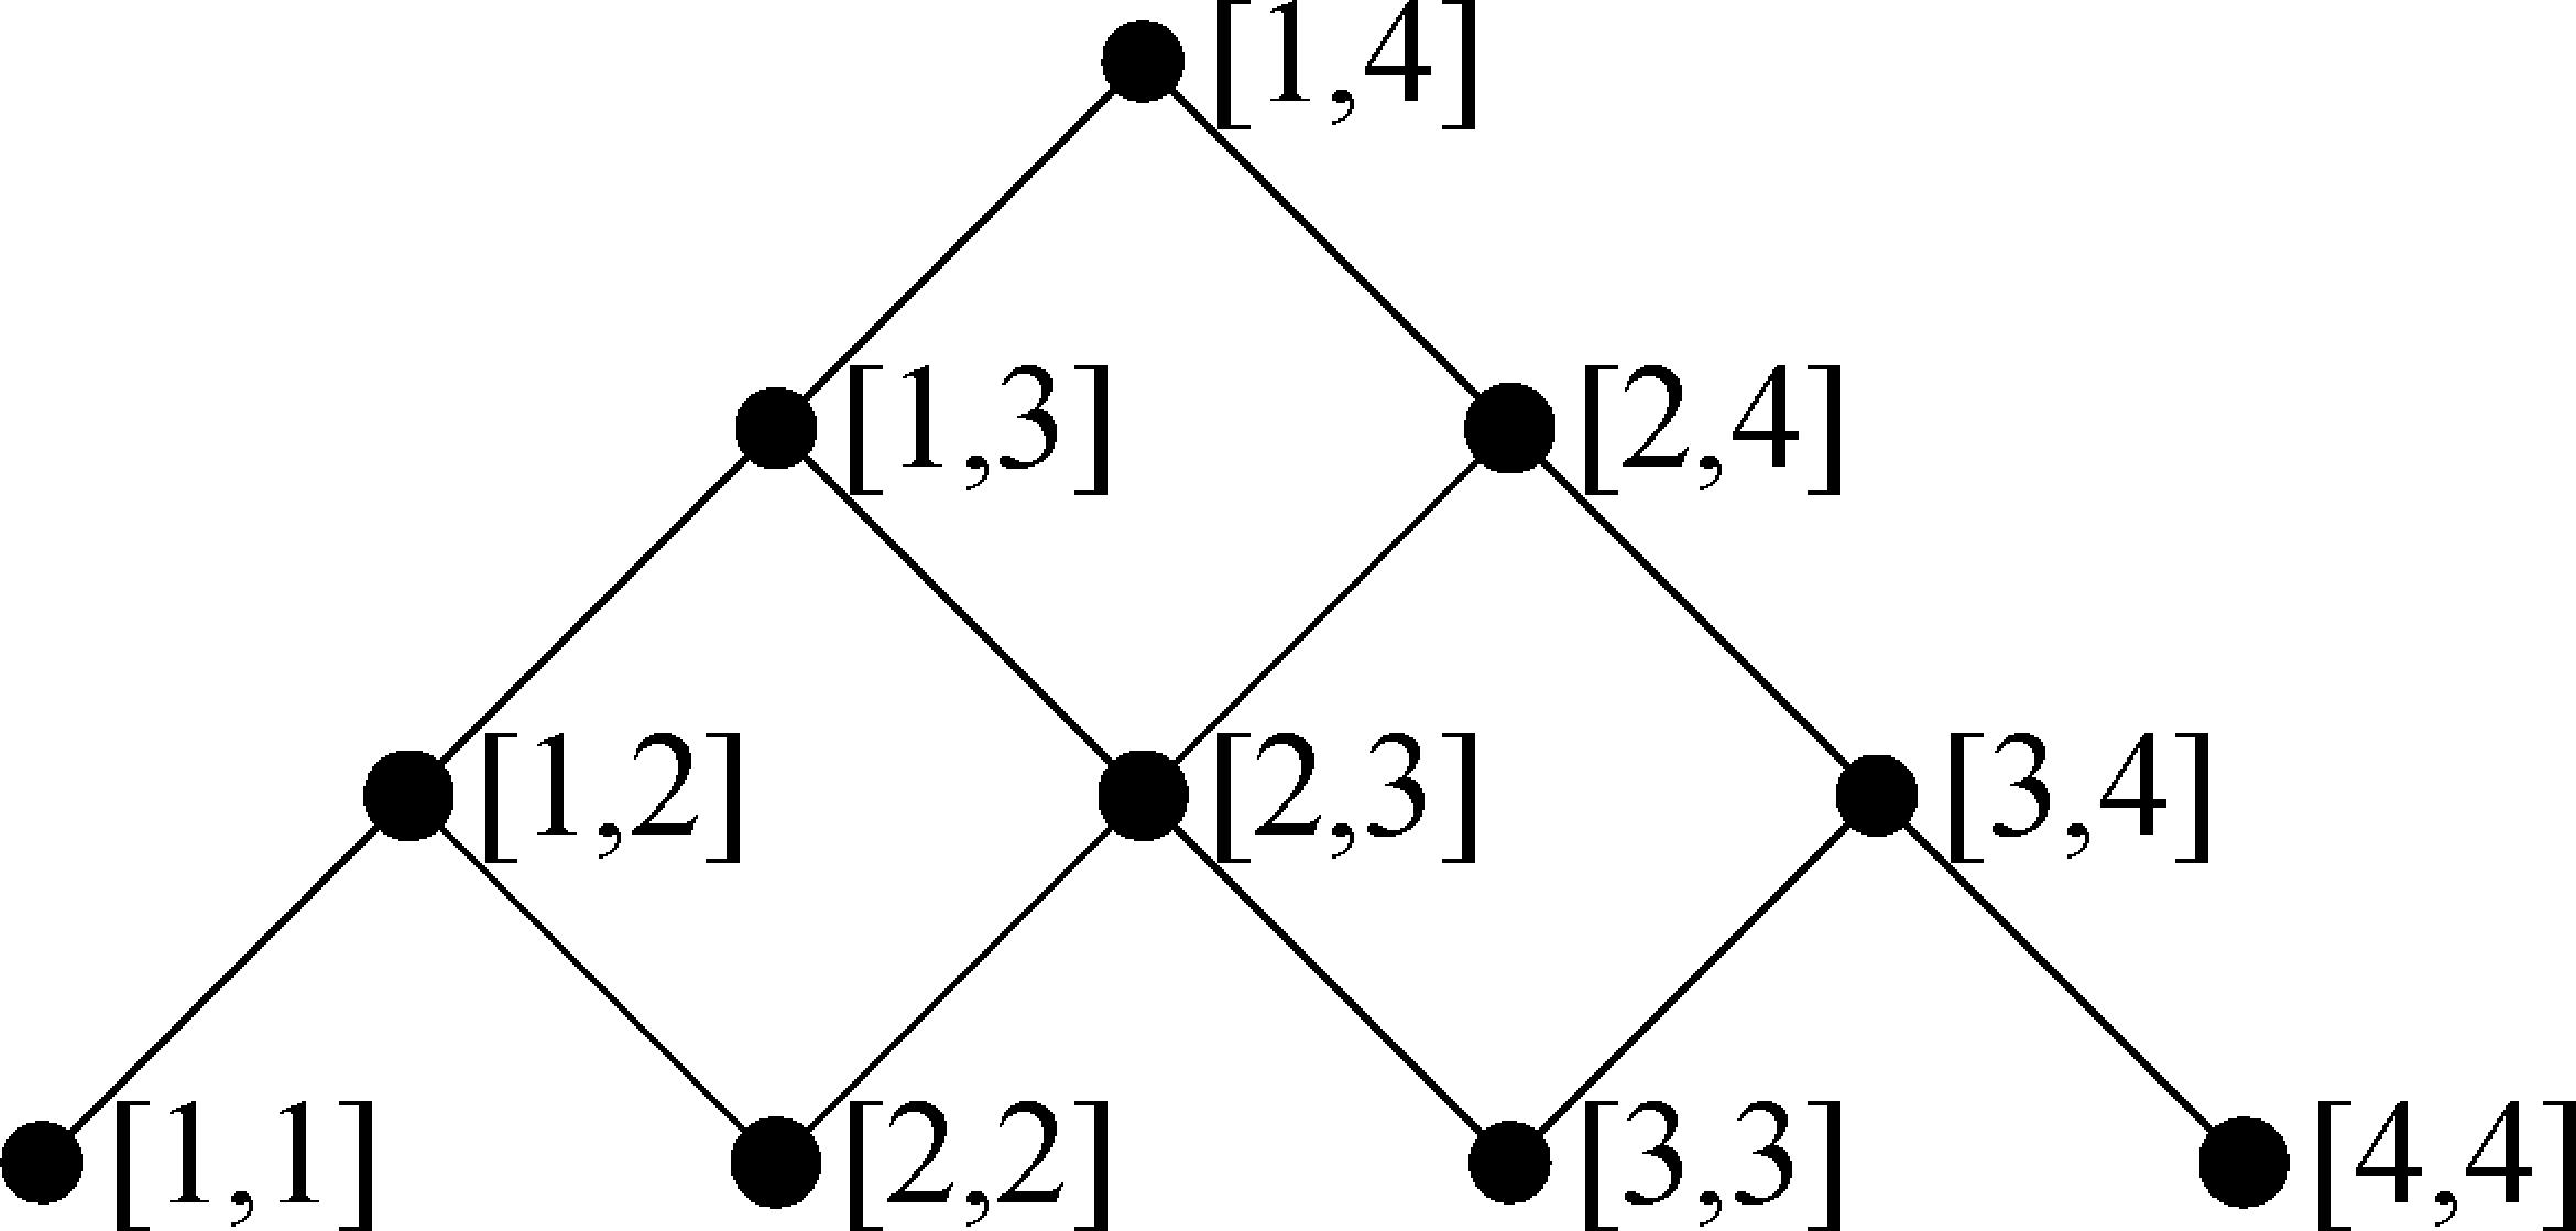
\includegraphics[scale=0.1]{images/lowerBounds/hasse.pdf}
  	\end{center}
  	\vspace*{1cm}
  	\tiny{Image source: Jason Crampton, ``Practical and Efficient Cryptographic Enforcement of Interval-Based Access Control Policies'', 2011.}

  \end{frame}
  
\end{document}